% Options for packages loaded elsewhere
\PassOptionsToPackage{unicode}{hyperref}
\PassOptionsToPackage{hyphens}{url}
%
\documentclass[
  11pt,
  letterpaper,
]{book}
\usepackage{lmodern}
\usepackage{amssymb,amsmath}
\usepackage{ifxetex,ifluatex}
\ifnum 0\ifxetex 1\fi\ifluatex 1\fi=0 % if pdftex
  \usepackage[T1]{fontenc}
  \usepackage[utf8]{inputenc}
  \usepackage{textcomp} % provide euro and other symbols
\else % if luatex or xetex
  \usepackage{unicode-math}
  \defaultfontfeatures{Scale=MatchLowercase}
  \defaultfontfeatures[\rmfamily]{Ligatures=TeX,Scale=1}
\fi
% Use upquote if available, for straight quotes in verbatim environments
\IfFileExists{upquote.sty}{\usepackage{upquote}}{}
\IfFileExists{microtype.sty}{% use microtype if available
  \usepackage[]{microtype}
  \UseMicrotypeSet[protrusion]{basicmath} % disable protrusion for tt fonts
}{}
\makeatletter
\@ifundefined{KOMAClassName}{% if non-KOMA class
  \IfFileExists{parskip.sty}{%
    \usepackage{parskip}
  }{% else
    \setlength{\parindent}{0pt}
    \setlength{\parskip}{6pt plus 2pt minus 1pt}}
}{% if KOMA class
  \KOMAoptions{parskip=half}}
\makeatother
\usepackage{xcolor}
\IfFileExists{xurl.sty}{\usepackage{xurl}}{} % add URL line breaks if available
\IfFileExists{bookmark.sty}{\usepackage{bookmark}}{\usepackage{hyperref}}
\hypersetup{
  pdftitle={Modélisation statistique},
  hidelinks,
  pdfcreator={LaTeX via pandoc}}
\urlstyle{same} % disable monospaced font for URLs
\usepackage{longtable,booktabs}
% Correct order of tables after \paragraph or \subparagraph
\usepackage{etoolbox}
\makeatletter
\patchcmd\longtable{\par}{\if@noskipsec\mbox{}\fi\par}{}{}
\makeatother
% Allow footnotes in longtable head/foot
\IfFileExists{footnotehyper.sty}{\usepackage{footnotehyper}}{\usepackage{footnote}}
\makesavenoteenv{longtable}
\usepackage{graphicx}
\makeatletter
\def\maxwidth{\ifdim\Gin@nat@width>\linewidth\linewidth\else\Gin@nat@width\fi}
\def\maxheight{\ifdim\Gin@nat@height>\textheight\textheight\else\Gin@nat@height\fi}
\makeatother
% Scale images if necessary, so that they will not overflow the page
% margins by default, and it is still possible to overwrite the defaults
% using explicit options in \includegraphics[width, height, ...]{}
\setkeys{Gin}{width=\maxwidth,height=\maxheight,keepaspectratio}
% Set default figure placement to htbp
\makeatletter
\def\fps@figure{htbp}
\makeatother
\setlength{\emergencystretch}{3em} % prevent overfull lines
\providecommand{\tightlist}{%
  \setlength{\itemsep}{0pt}\setlength{\parskip}{0pt}}
\setcounter{secnumdepth}{5}
\usepackage{mathtools}
\usepackage{enumerate}
\usepackage{geometry}
\usepackage[french]{babel}
\geometry{hmargin=1.2in}
% \usepackage[mathscr]{eucal}
\usepackage{fontspec}
\setmainfont[Scale=0.925]{heuristica}
\usepackage[scr=rsfs]{mathalpha}
% \DeclareMathAlphabet{\mathcrl}{U}{rsfs}{m}{n}
% \DeclareMathAlphabet{\mathcal}{OMS}{cmsy}{m}{n}
% \usepackage{booktabs} % already loaded
\usepackage{amsthm}
\makeatletter
\def\thm@space@setup{%
  \thm@preskip=8pt plus 2pt minus 4pt
  \thm@postskip=\thm@preskip
}
\makeatother
\usepackage{framed,color}
\definecolor{shadecolor}{RGB}{248,248,248}

\renewcommand{\textfraction}{0.05}
\renewcommand{\topfraction}{0.8}
\renewcommand{\bottomfraction}{0.8}
\renewcommand{\floatpagefraction}{0.75}

\let\oldhref\href
\renewcommand{\href}[2]{#2\footnote{\url{#1}}}

\ifxetex
  \usepackage{letltxmacro}
  \setlength{\XeTeXLinkMargin}{1pt}
  \LetLtxMacro\SavedIncludeGraphics\includegraphics
  \def\includegraphics#1#{% #1 catches optional stuff (star/opt. arg.)
    \IncludeGraphicsAux{#1}%
  }%
  \newcommand*{\IncludeGraphicsAux}[2]{%
    \XeTeXLinkBox{%
      \SavedIncludeGraphics#1{#2}%
    }%
  }%
\fi

\makeatletter
\newenvironment{kframe}{%
\medskip{}
\setlength{\fboxsep}{.8em}
 \def\at@end@of@kframe{}%
 \ifinner\ifhmode%
  \def\at@end@of@kframe{\end{minipage}}%
  \begin{minipage}{\columnwidth}%
 \fi\fi%
 \def\FrameCommand##1{\hskip\@totalleftmargin \hskip-\fboxsep
 \colorbox{shadecolor}{##1}\hskip-\fboxsep
     % There is no \\@totalrightmargin, so:
     \hskip-\linewidth \hskip-\@totalleftmargin \hskip\columnwidth}%
 \MakeFramed {\advance\hsize-\width
   \@totalleftmargin\z@ \linewidth\hsize
   \@setminipage}}%
 {\par\unskip\endMakeFramed%
 \at@end@of@kframe}
\makeatother

\makeatletter
\@ifundefined{Shaded}{
}{\renewenvironment{Shaded}{\begin{kframe}}{\end{kframe}}}
\makeatother

\newenvironment{rmdblock}[1]
  {
  \begin{itemize}
  \renewcommand{\labelitemi}{
    \raisebox{-.7\height}[0pt][0pt]{
      {\setkeys{Gin}{width=3em,keepaspectratio}\includegraphics{images/#1}}
    }
  }
  \setlength{\fboxsep}{1em}
  \begin{kframe}
  \item
  }
  {
  \end{kframe}
  \end{itemize}
  }
\newenvironment{rmdnote}
  {\begin{rmdblock}{note}}
  {\end{rmdblock}}
\newenvironment{rmdcaution}
  {\begin{rmdblock}{caution}}
  {\end{rmdblock}}
\newenvironment{rmdimportant}
  {\begin{rmdblock}{important}}
  {\end{rmdblock}}
\newenvironment{rmdtip}
  {\begin{rmdblock}{tip}}
  {\end{rmdblock}}
\newenvironment{rmdwarning}
  {\begin{rmdblock}{warning}}
  {\end{rmdblock}}
\usepackage[]{natbib}
\bibliographystyle{apalike2}

\title{Modélisation statistique}
\author{}
\date{\vspace{-2.5em}}

\begin{document}
\maketitle

\let\href\oldhref

{
\setcounter{tocdepth}{1}
\tableofcontents
}
\hypertarget{remarques}{%
\chapter*{Remarques}\label{remarques}}
\addcontentsline{toc}{chapter}{Remarques}

Ces notes sont l'oeuvre de Léo Belzile (HEC Montréal) et sont mis à disposition sous la \href{https://creativecommons.org/licenses/by-nc-sa/4.0/legalcode.fr}{Licence publique Creative Commons Attribution - Utilisation non commerciale - Partage dans les mêmes conditions 4.0 International} et ont été compilé le 25 juin 2020.

Bien que les diapositives illustrent l'implémentation des techniques statistiques et des modèles à l'aide de \textbf{SAS}, ces notes présentent le pendant \textbf{R}: visitez \href{https://cran.r-project.org/}{le site web du projet \textbf{R}} pour télécharger le logiciel. L'interface graphique la plus populaire (et celle que je vous recommande) est \href{https://www.rstudio.com/products/rstudio/download/}{RStudio Desktop}.

\newcommand{\bs}[1]{\boldsymbol{#1}}
\newcommand{\Hmat}{\mathbf{H}}
\newcommand{\Mmat}{\mathbf{M}}
\newcommand{\mX}{\mathbf{X}}
\newcommand{\bX}{{\mathbf{X}}}
\newcommand{\bx}{{\mathbf{x}}}
\newcommand{\by}{{\boldsymbol{y}}}
\newcommand{\bY}{{\boldsymbol{Y}}}
\newcommand{\eps}{\varepsilon}
\newcommand{\beps}{\boldsymbol{\varepsilon}}
\newcommand{\bbeta}{\boldsymbol{\beta}}
\newcommand{\hbb}{\widehat{\boldsymbol{\beta}}}
\newcommand{\limni}{\lim_{n \ra \infty}}
\newcommand{\pr}{{\mathsf Pr}{}}
\newcommand{\E}[2][]{{\mathsf E}_{#1}\left(#2\right)}
\newcommand{\Va}[2][]{{\mathsf{Var}_{#1}}\left(#2\right)}
\newcommand{\I}[1]{{\mathbf 1}_{#1}}
\renewcommand{\d}{\mathrm{d}}

\hypertarget{intro}{%
\chapter{Introduction à l'inférence statistique}\label{intro}}

\hypertarget{pruxe9requis}{%
\section{Prérequis}\label{pruxe9requis}}

Bien que sans prérequis, nous assumerons que l'étudiant(e) a une connaissance préalable des notions suivantes:

\begin{itemize}
\tightlist
\item
  population et échantillon,
\item
  types de variables: continues, catégorielles (ordinales ou nominales), binaires,
\item
  variables aléatoires et leurs lois (Bernoulli, binomiale, géométrique, Poisson, normale, Student, exponentielle, Weibull, etc.),
\item
  propriétés de variables aléatoires: espérance, variance, biais,
\item
  graphiques de base (histogramme, nuage de point, densité, boîte à moustache, etc.),
\item
  tests d'hypothèses, puissance et erreur de type I,
\item
  théorème central limite,
\item
  valeurs-\(p\) et intervalles de confiance,
\item
  tests-\(t\) pour un et deux échantillons et pour données appariées,
\item
  régression linéaire simple.
\end{itemize}

Ces notions sont d'ordinaire traitées dans un cours d'introduction à la statistique au niveau baccalauréat/licence, voir même au collégial.

L'inférence statistique a pour but de tirer des conclusions formelles à partir de données. Dans le cadre de la recherche scientifique, le chercheur formule une hypothèse, collecte des données pour valider ou infirmer cette dernière et conclure quant à la plausibilité de son hypothèse.

On distingue deux types de jeux de données: les données \textbf{expérimentales} sont typiquement collectées en milieu contrôlé suivant un protocole d'enquête et un plan d'expérience: elles servent à répondre à une question prédéterminée. L'approche expérimentale est désirable pour éviter le «jardin des embranchements» (une \href{http://www.stat.columbia.edu/~gelman/research/unpublished/p_hacking.pdf}{allégorie signifiant qu'un chercheur peut raffiner son hypothèse à la lumière des données, sans ajustement pour des variables confondantes}), mais elle n'est pas toujours réalisable: par exemple, un économiste ne peut pas modifier les taux d'intérêts pour observer les impacts sur le taux d'épargne des consommateurs. Lorsque les données ont déjà été collectées, on parle de données \textbf{observationnelles}.

On fera dans ce cours une distinction entre inférence et prédiction, bien que ces deux objectifs ne soient pas mutuellement exclusifs. La plupart des boîtes noires utilisées en apprentissage automatique tombent dans la catégorie des modèles prédictifs: ces modèles ne sont pas interprétables et ignorent parfois la structure inhérente aux données. Par contraste, les modèles explicatifs qui servent à l'inférence sont souvent simples et interprétables.

Ce chapitre porte sur deux concepts fondamentaux pour la modélisation, à savoir les principes sous-jacents aux tests d'hypothèses et l'analyse exploratoire des données. Il contient également des exemples de problèmes quotidiens pour lesquels la statistique offre des pistes de réflexion.

Plusieurs exemples seront traités dans le cours:

\begin{itemize}
\tightlist
\item
  Est-ce qu'il y a de la discrimination salariale envers les femmes professeurs d'un collège américain?
\item
  Quels sont les critères médicaux qui impactent les primes d'assurance maladies?
\item
  Qu'est-ce qui explique que les prix de l'essence soient plus élevés en Gaspésie qu'ailleurs au Québec? \href{http://www.regie-energie.qc.ca/energie/rapports/Rapport_PrixGasp\%C3\%A9sie_20191219.pdf}{Un rapport de surveillance des prix de l'essence en Gaspésie par la Régie de l'énergie se penche sur la question.}
\item
  Est-ce que les examens pratiques de conduite sont plus faciles en régions en Grande-Bretagne? \href{https://www.theguardian.com/world/2019/aug/23/an-easy-ride-scottish-village-fuels-debate-driving-test-pass-rates}{Une analyse du journal britannique \emph{The Guardian}} laisse penser que c'est le cas.
\item
  Est-ce le risque de transmission de la Covid augmente en fonction de la distanciation? \href{https://www.thelancet.com/journals/lancet/article/PIIS0140-6736(20)31142-9/fulltext}{Une (mauvaise) méta-analyse souligne que c'est le cas} (ou l'art de tirer des conclusions erronées à partir d'une étude bancale).
\end{itemize}

\hypertarget{tests-dhypothuxe8se-heuristique}{%
\section{Tests d'hypothèse (heuristique)}\label{tests-dhypothuxe8se-heuristique}}

Un test d'hypothèse statistique est une façon d'évaluer la preuve statistique provenant d'un échantillon afin de faire une décision quant à la population sous-jacente. Les étapes principales sont:

\begin{itemize}
\tightlist
\item
  définir les hypothèses que l'on veut tester en fonction de paramètres du modèle,
\item
  calculer la statistique de test,
\item
  déterminer son comportement sous \(\mathscr{H}_0\) (loi nulle),
\item
  calculer la valeur-\(p\),
\item
  conclure dans le contexte du problème (rejeter ou ne pas rejeter \(\mathscr{H}_0\)).
\end{itemize}

Mon approche privilégiée pour présenter les tests d'hypothèse est de faire un parallèle avec un procès pour meurtre où vous êtes nommé juré.

\begin{itemize}
\tightlist
\item
  Le juge vous demande de choisir entre deux hypothèses mutuellement exclusives, coupable ou non-coupable, sur la base des preuves présentées.
\item
  Votre postulat de départ repose sur la présomption d'innocence: vous condamnerez uniquement le suspect si la preuve est accablante. Cela permet d'éviter les erreurs judiciaires. L'hypothèse nulle \(\mathscr{H}_0\) est donc \emph{non-coupable}, et l'hypothèse alternative \(\mathscr{H}_a\) est coupable. En cas de doute raisonnable, vous émettrez un verdict de non-culpabilité.
\item
  La preuve présentée est la statistique de test. La couronne choisit la preuve de manière à appuyer son postulat de culpabilité le mieux possible. Ce choix reflète la \textbf{puissance} (plus la preuve est accablante, plus grande est la chance d'un verdict de culpabilité --- le procureur a donc tout intérêt à bien choisir les faits présentés en cour).
\item
  En qualité de juré, vous analysez la preuve à partir de la jurisprudence et de l'avis d'expert pour vous assurer que les faits ne relèvent pas du hasard. Pour le test d'hypothèse, ce rôle est tenu par la loi sous \(\mathscr{H}_0\): si la personne était innocente, est-ce que les preuves présentées tiendraient la route? Des preuves probantes (ADN, etc.) auront davantage de poids que des preuves circonstancielles (la pièce de théâtre \emph{Douze hommes en colère} de Reginald Rose présente un bel exemple de procès où un des juré émet un doute raisonnable et convainc un à un les autres membres du jury de prononcer un verdict de non-culpabilité).
\item
  Vous émettez un verdict, à savoir une décision binaire, où l'accusé est déclaré soit non-coupable, soit coupable. Si vous avez une valeur-\(p\), disons \(P\), pour votre statistique de test et que vous effectuez ce dernier à niveau \(\alpha\), la règle de décision revient à rejeter \(\mathscr{H}_0\) si \(P < \alpha\).
\end{itemize}

On s'attarde davantage sur ces définitions heuristiques et le vocabulaire employé pour parler de tests d'hypothèse. Le matériel de la section suivante a été préparé par Juliana Schulz.

\hypertarget{hypothuxe8se}{%
\subsection{Hypothèse}\label{hypothuxe8se}}

Dans les test statistique il y a toujours deux hypothèse: l'hypothèse nulle (\(\mathscr{H}{}_{0}\)) et l'hypothèse alternative (\(\mathscr{H}_a\)). Habituellement, l'hypothèse nulle est le « statu quo » et l'alternative est l'hypothèse que l'on cherche à démontrer. Un test d'hypothèse statistique nous permet de décider si nos données nous fournissent assez de preuves pour rejeter \(\mathscr{H}_0\) en faveur de \(\mathscr{H}_a\), selon un risque d'erreur spécifié. Généralement, les tests d'hypothèses sont exprimés en fonction de paramètres (de valeurs inconnues) du modèle sous-jacent, par ex. \(\theta\). Un test d'hypothèse bilatéral concernant un paramètre unidimensionnel \(\theta\) s'exprimerait la forme suivante:
\begin{align*}
\mathscr{H}_0: \theta=\theta_0 \qquad \text{versus} \qquad \mathscr{H}_a:\theta \neq \theta_0.
\end{align*}
Ces hypothèses permettent de tester si \(\theta\) est égal précisément à une valeur, \(\theta_0\).

Par exemple, pour un test bilatéral concernant le paramètre d'un modèle de régression \(\beta_j\) associé à une variable explicative d'intérêt \(\mathrm{X}_j\) dans la population, les hypothèses sont:
\begin{align*}
\mathscr{H}_0: \beta_j=\beta_j^0 \qquad \text{versus} \qquad \mathscr{H}_a:\beta_j \neq \beta_j^0, 
\end{align*}
où \(\beta_j^0\) est une valeur précise qui est reliée à la question de recherche. Par exemple, si \(\beta_j^0=0\) la question de recherche sous-jacente est: est-ce que la covariable \(\mathrm{X}_j\) impacte la variable réponse d'intérêt \(Y\)?

Remarque: il est possible d'imposer une direction dans les tests en considérant une hypothèse alternative de la forme \(\mathscr{H}_a: \theta > \theta_0\) ou \(\mathscr{H}_a: \theta < \theta_0\).

\hypertarget{statistique-de-test}{%
\subsection{Statistique de test}\label{statistique-de-test}}

Une statistique de test \(T\) est une fonction des données d'échantillon qui contient de résume l'information contenue dans les données pour \(\theta\). La forme de la statistique de test est choisie de façon à ce que son comportement sous \(\mathscr{H}_0\), c'est-à-dire l'ensemble des valeurs que prend \(T\) si \(\mathscr{H}_0\) est vraie et leur probabilité relative, soit connu. En effet, \(T\) est une variable aléatoire et sa valeur va changer selon l'échantillon. La \textbf{loi nulle} de la statistique de test nous permet de déterminer quelles valeurs de \(T\) sont plausibles si \(\mathscr{H}_0\) est vraie. Plusieurs statistiques que l'on couvrira dans ce cours sont des \textbf{statistiques de Wald}, de la forme
\begin{align*}
T = \frac{\widehat{\theta} - \theta_0}{\mathrm{se}(\widehat{\theta})} 
\end{align*}
où \(\widehat{\theta}\) est l'estimateur du paramètre \(\theta\) et \(\mathrm{se}(\widehat{\theta})\) est l'estimateur de l'écart-type de \(\widehat{\theta}\).

Un \textbf{estimateur} est une règle ou une formule utilisée pour calculer l'estimation d'un paramètre ou quantité d'intérêt selon des données observées. Par exemple, la moyenne d'échantillon \(\overline{X}\) est un estimateur de la moyenne dans la population \(\mu\). Une fois qu'on a des données observées, on peut calculer la valeur de \(\overline{X}\), c'est-à-dire, on obtient une valeur numérique, appelée estimé. Autrement dit, un estimateur est la procédure ou formule qui nous dit comment utiliser les données pour calculer une estimation. Un estimateur est une variable aléatoire car sa valeur dépend sur l'échantillon. L'estimé, quant à lui, est la valeur numérique calculée sur un échantillon donné.

Par exemple, pour une hypothèse sur la moyenne d'une population de la forme
\begin{align*}
\mathscr{H}_0: \mu=0 \qquad \text{versus} \qquad \mathscr{H}_a:\mu \neq 0, 
\end{align*}
la statistique de test de Wald est
\begin{align*}
T &= \frac{\overline{X}-0}{S_n/\sqrt{n}}
\end{align*}
où \(\overline{X}\) est la moyenne de l'échantillon \(X_1, \ldots, X_n\),
\begin{align*}
\overline{X} &= \frac{1}{n} \sum_{i=1}^n X_i
\end{align*}
et l'erreur-type de la moyenne \(\overline{X}\) est \(S_n/\sqrt{n}\); l'écart-type \(S_n\) est un estimateur de \(\sigma\), où
\begin{align*}
S^2_n &= \frac{1}{n-1} \sum_{i=1}^n (X_i-\overline{X})^2.
\end{align*}

\hypertarget{loi-nulle-et-valeur-p}{%
\subsection{\texorpdfstring{Loi nulle et valeur-\(p\)}{Loi nulle et valeur-p}}\label{loi-nulle-et-valeur-p}}

La \textbf{valeur-\(p\)} nous permet de déterminer si la valeur observée de la statistique de test \(T\) est plausible sous \(\mathscr{H}_0\). Plus précisément, la valeur-\(p\) est la probabilité que la statistique de test est égal or encore plus extrême de ce qu'on observe selon les données, en supposant que \(\mathscr{H}_0\) est vraie. Suppose qu'on a un échantillon \(X_1, \ldots, X_n\) et qu'on observe une valeur de la statistique de test de \(T=t\). Pour un test d'hypothèse bilatéral \(\mathscr{H}_0:\theta=\theta_0\) vs.~\(\mathscr{H}_a:\theta \neq \theta_0\), la valeur-\(p\) est
\(\mathsf{Pr}_0(|T| \geq |t|)\), c'est-à-dire, la probabilité que \(|T|\) est égal ou plus grand que ce qu'on observe, en valeur absolue, sous \(\mathscr{H}_0\). Si la distribution de \(T\) est symétrique autour de \(0\), la valeur-\(p\) vaut
\begin{align*}
p = 2 \times \mathsf{Pr}_0(T \geq |t|), 
\end{align*}

Prenons l'exemple d'un test d'hypothèse bilatéral pour la moyenne au population \(\mathscr{H}_0:\mu=0\) contre \(\mathscr{H}_a:\mu \neq 0\). Si l'échantillon provient d'une (population de) loi normale \(\mathsf{No}(\mu, \sigma^2)\), on peut démontrer que, si \(\mathscr{H}_0\) est vraie et donc, \(\mu=0\)), la statistique de test
\begin{align*}
T = \frac{\overline{X}}{S/\sqrt{n}}
\end{align*}
suit une loi de Student-\(t\) avec \(n-1\) degrés de liberté. Avec cette loi nulle, on peut calculer la valeur-\(p\) (ou bien à partir d'une table ou en utilisant un logiciel statistique). Puisque la distribution Student-\(t\) est symétrique autour de \(0\), on peut calculer la valeur-\(p\) comme \(P = 2\times\mathsf{Pr}(T_{n-1} > |t|)\), où \(T_{n-1}\) dénote une variable aléatoire avec distribution de Student-\(t\) avec \(n-1\) degrés de liberté.

\hypertarget{conclusion}{%
\subsection{Conclusion}\label{conclusion}}

La valeur-\(p\) nous permet de faire une décision quant aux hypothèses du test. Si \(\mathscr{H}_0\) est vraie, la valeur-\(p\) suit une loi uniforme. Si la valeur-\(p\) est petite, ça veut dire que le fait d'observer une statistique de test égal ou encore plus extrême que \(t\) est peu probable, et donc nous aurons tendance de croire que \(\mathscr{H}_0\) n'est pas vraie. Il y a pourtant toujours un risque sous-jacent qu'on fait un erreur quand on fait une décision. En statistique, il y a deux types d'erreurs:

\begin{itemize}
\tightlist
\item
  erreur de type I: on rejette \(\mathscr{H}_0\) alors que \(\mathscr{H}_0\) est vraie
\item
  erreur de type II: on ne rejette pas \(\mathscr{H}_0\) alors que \(\mathscr{H}_0\) est fausse
\end{itemize}

Si le modèle générant les données est correct (sic), alors l'hypothèse nulle ou l'hypothèse alternative est vraie (ces deux scénarios couvrant l'univers des possibles).

\begin{longtable}[]{@{}lcc@{}}
\toprule
Décision\textbackslash{} vrai modèle & \(\mathscr{H}_0\) & \(\mathscr{H}_a\)\tabularnewline
\midrule
\endhead
ne pas rejeter \(\mathscr{H}_0\) & \(\checkmark\) & erreur de type II\tabularnewline
rejeter \(\mathscr{H}_0\) & erreur de type I & \(\checkmark\)\tabularnewline
\bottomrule
\end{longtable}

Comme chercheur, on doit fixer préalablement le niveau de risque que nous sommes prêt à tolérer. Si on connaît la distribution de \(T\) sous \(\mathscr{H}_0\), on peut contrôler le risque de faire un erreur de type I. Ceci fait référence au \textbf{niveau} du test, dénoté par \(\alpha\):
\begin{align*}
\alpha = \mathsf{P}_0\left(\text{ rejeter } \mathscr{H}_0\right).
\end{align*}
La valeur de \(\alpha \in (0, 1)\) est la probabilité qu'on rejette \(\mathscr{H}_0\) quand \(\mathscr{H}_0\) est en fait vraie. Comme chercheur, on choisit ce niveau \(\alpha\); habituellement \(1\)\%, \(5\)\% ou \(10\)\%. Pour prendre une décision, on doit comparer la valeur-\(p\) \(P\) avec le niveau du test \(\alpha\):

\begin{itemize}
\tightlist
\item
  si \(P < \alpha\) on rejette \(\mathscr{H}_0\),
\item
  si \(P \geq \alpha\) on ne rejette pas \(\mathscr{H}_0\).
\end{itemize}

\hypertarget{puissance-statistique}{%
\subsection{Puissance statistique}\label{puissance-statistique}}

Quand on ne rejette pas \(\mathscr{H}_0\) et que \(\mathscr{H}_a\) est en fait vraie, on fait un erreur de type II. Dénotons par \(1-\gamma\) la probabilité de faire une erreur de type II, c'est-à-dire
\begin{align*}
\gamma = \mathsf{Pr}_a(\text{rejeter } \mathscr{H}_0)
\end{align*}
La \textbf{puissance statistique} d'un test est la probabilité que le test rejette \(\mathscr{H}_0\) alors que \(\mathscr{H}_0\) est fausse, soit \(\gamma\). On veut qu'un test ait une puissance élevée, c'est-à-dire, on veut que \(\gamma\) soit le plus près de 1 possible. Minimalement, la puissance du test devrait être \(\alpha\) parce qu'on rejette \(\alpha\) pourcent du temps même quand l'hypothèse nulle est vraie. La variabilité des données et la taille de l'écart réel dans la population influent sur la puissance, mais nous n'avons pas de contrôle sur ces paramètres. À l'inverse, on peut augmenter la taille de l'échantillon pour augmenter la puissance. Le choix de la statistique de test influe aussi sur la puissance, mais les statistiques de test que nous choisirons sont souvent standard et parmi les plus puissantes qui soient, aussi on ne traitera pas de ce point dans le cadre de ce cours.

\hypertarget{intervalle-de-confiance}{%
\subsection{Intervalle de confiance}\label{intervalle-de-confiance}}

Un \textbf{intervalle de confiance} est une manière alternative de rapporter les conclusions d'un test, en ce sent qu'on fournit une estimation ponctuelle de \(\hat{\theta}\) avec une marge d'erreur. L'intervalle de confiance donne donc une indication de la variabilité de la procédure d'estimation. Un intervalle de confiance de Wald à \((1-\alpha)\) pour un paramètre \(\theta\) est de la forme
\begin{align*}
\widehat{\theta} \pm \mathfrak{q}_{\alpha/2} \; \mathrm{se}(\widehat{\theta})
\end{align*}
où \(\mathfrak{q}_{\alpha/2}\) est le quantile d'ordre \(1-\alpha/2\) de la loi nulle de la statistique de Wald \(T\), soit
\begin{align*}
T =\frac{\widehat{\theta}-\theta}{\mathrm{se}(\widehat{\theta})}
\end{align*}
et \(\theta\) représente la valeur du paramètre \(\theta\) (supposé fixe, mais inconnu) de la population. Les bornes de l'intervalle de confiance sont aléatoires puisque \(\widehat{\theta}\) et \(\mathrm{se}(\widehat{\theta})\) sont des variable aléatoires: leurs valeurs dépend sur l'échantillon et donc varient d'un échantillon à un autre.

Par exemple, pour un échantillon aléatoire \(X_1, \ldots, X_n\) provenant d'une loi normale \(\mathsf{No}(\mu, \sigma)\), l'intervalle de confiance à \((1-\alpha)\) pour la moyenne (dans la population) \(\mu\) est
\begin{align*}
\overline{X} \pm t_{n-1, \alpha/2} \frac{S}{\sqrt{n}}
\end{align*}
où \(t_{n-1, \alpha/2}\) est le quantile d'ordre \(1-\alpha/2\) de la loi Student-\(t\) avec \(n-1\) degrés de libertés.

Avant qu'on calcule l'intervalle de confiance, il y a une probabilité de \(1-\alpha\) que \(\theta\) soit contenu dans l'intervalle \textbf{aléatoire} symmétrique \((\widehat{\theta} - \mathfrak{q}_{\alpha/2} \; \mathrm{se}(\widehat{\theta}), \widehat{\theta} + \mathfrak{q}_{\alpha/2} \; \mathrm{se}(\widehat{\theta}))\). Une fois qu'on a un échantillon et qu'on calcule les bornes de l'intervalle de confiance, il n'y a plus de notion de probabilité. La vraie valeur du paramètre \(\theta\) est soit contenue dans l'intervalle de confiance, soit pas. La seule interprétation de l'intervalle de confiance qui soit valable alors est la suivante: si on répète l'expérience plusieurs fois et qu'à chaque fois on calcule un intervalle de confiance à \(1-\alpha\), alors \(1-\alpha\) de ces intervalles devraient contenir la vraie valeur de \(\theta\) (de la même manière, si vous lancez une pièce de monnaie équilibrée, vous devriez obtenir une fréquence de 50\% de pile et 50\% de face, mais chaque lancer donnera un ou l'autre de ces choix).

\begin{figure}

{\centering 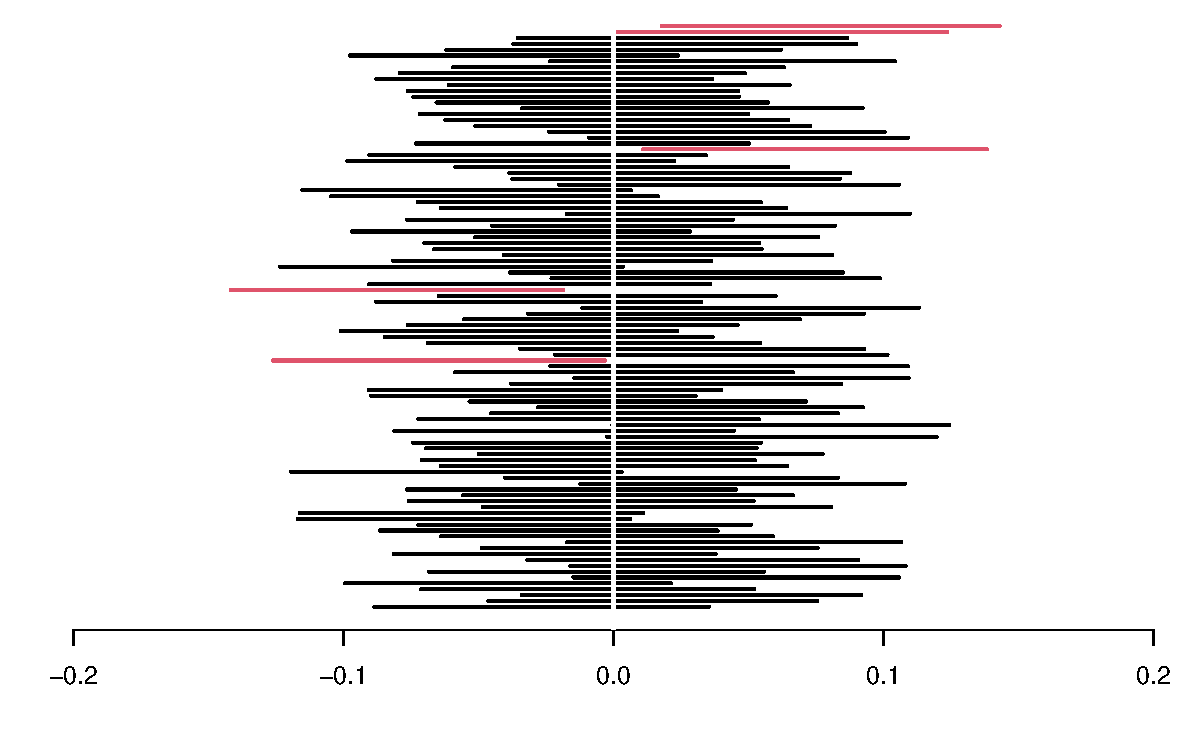
\includegraphics[width=0.7\linewidth]{MATH60604_Modelisation_statistique_files/figure-latex/intconf-1} 

}

\caption{Intervalles de confiance à 95\% pour la moyenne d'une population normale $\mathsf{No}(0,1)$. Environ 95 de ces 100 intervalles devraient inclure zéro.}\label{fig:intconf}
\end{figure}

L'intervalle de confiance peut être considéré comme le pendant du test d'hypothèse. À niveau \(\alpha\), on ne rejetterait aucune des valeurs contenues dans l'intervalle de confiance de niveau \(1-\alpha\). Si la valeur-\(p\) est inférieure à \(\alpha\), la valeur postulée pour \(\theta\) est donc hors intervalle. La valeur-\(p\) ne donne la probabilité que pour une valeur postulée, mais permet de quantifier à quel point le résultat est extrême.

\hypertarget{exemple-achat-en-ligne-de-milluxe9niaux}{%
\subsection{Exemple: achat en ligne de milléniaux}\label{exemple-achat-en-ligne-de-milluxe9niaux}}

Supposons qu'un chercheur veut faire une étude sur l'évolution des ventes en ligne au Canada. Elle postule que la génération Y (les milléniaux) font plus d'achats en ligne que les générations antérieures. Pour répondre à cette question, un sondage est envoyé à un échantillon aléatoire de \(n=500\) individus représentatif de la population avec 160 milléniaux et 340 personnes plus âgées issues des générations X et des baby-boomers. La variable \texttt{depenses} mesure le montant d'achat effectués en ligne dans le mois dernier (en dollars).

On pourrait simplement considérer la différence entre le montant moyen des Y et celui des autres générations; on standardise par l'écart-type de l'échantillon pour obtenir une valeur sans unité de mesure. La différence de moyenne observée dans l'échantillon est de 16.49 dollars et donc les milléniaux ont dépensé davantage. En revanche, notre échantillon est aléatoire et le montant d'achat en ligne d'un individu à l'autre (et d'un mois à l'autre) est variable.

La première étape de notre analyse consiste à définir les quantités d'intérêt et à formuler nos hypothèse en fonction de paramètres du modèle; il convient également de définir ces derniers. Dans cet exemple, on considère un test pour la différence de moyenne dans les populations postulées \(\mu_1\) (pour la génération Y) et \(\mu_2\) (pour les générations antérieures) d'écart-type respectif \(\sigma_1\) et \(\sigma_2\). Comment déterminer quelle hypothèse on considère? Comme statisticien, on se fait l'avocat du Diable: l'hypothèse d'intérêt du chercheur est l'hypothèse alternative et ici, \(\mathscr{H}_a: \mu_1 > \mu_2\), où \(\mu_1\) représente la moyenne des achats mensuels des milléniaux. L'hypothèse nulle en toutes les autres valeurs, soit \(\mathscr{H}_0: \mu_1 \leq \mu_2\), mais il suffit de considérer le cas \(\mu_1=\mu_2\) (pourquoi?). S'il n'y a aucune différence de moyenne entre les groupes, alors \(\overline{X}_1-\overline{X}_2\) a moyenne zéro; la différence de moyenne a une variance de \(\sigma^2_1/n_1+\sigma^2_2/n_2\). Il y a toujours possibilité de commettre une erreur judiciaire (dit erreur de Type 1, c'est-à-dire de condamner un innocent ou rejeter \(\mathscr{H}_0\) alors que l'hypothèse nulle est vraie). Pour se prémunir de ce risque, on fixe préalablement un niveau de tolérance. On effectuera le test à niveau \(\alpha=0.05\); cela veut dire que, si \(\mathscr{H}_0\) est vraie, on commettra une erreur de type I en moyenne cinq fois sur 100. Plus on choisit un \(\alpha\) petit, moins on arrivera à détecter quand l'hypothèse nulle est fausse (rappelez-vous que nous sommes intéressés à démontrer que l'hypothèse alternative).

La deuxième étape consiste à choisir une statistique de test. Ici, on considère la statistique de Welch (\citet{Welch:1947}) pour une différence de moyenne entre deux échantillons:
\begin{align*}
T = \frac{\overline{X}_1 - \overline{X}_2}{\left(\frac{S_1^2}{n_1}+\frac{S_2^2}{n_2} \right)^{1/2}}, 
\end{align*}
où \(\overline{X}_i\) est la moyenne empirique dans l'échantillon \(i\) (\(i=1, 2\)) et \(S_i^2\) est la variance empirique et \(n_i\) la taille de l'échantillon du groupe \(i\). La statistique est utilisée pour calculer la différence de moyennes de deux échantillons de variance potentiellement différente. La valeur de la statistique dans l'échantillon est 2.76, mais on obtiendrait une valeur différente avec un autre échantillon. Il convient donc de déterminer si cette valeur est compatible avec notre hypothèse nulle en la comparant à la loi nulle sous \(\mathscr{H}_0\) de \(T\).

La troisième étape est l'obtention d'un étalon de mesure pour déterminer si notre résultat est extrême ou inattendu. Vous remarquerez que la statistique de Welch a moyenne zéro et variance un sous l'hypothèse nulle que \(\mu_1=\mu_2\): standardiser une statistique permet d'obtenir un objet dont on connaît le comportement pour de grands échantillons.
Asymptotiquement, \(T\) suit une loi normale \(\mathsf{No}(0, 1)\), mais il existe une meilleure approximation pour \(n\) petit; on compare le comportement de \(T\) à l'aide d'une loi de Student (approximation de \citet{Satterthwaite:1946}).

La dernière étape consiste à obtenir une valeur-\(p\), soit la probabilité d'observer un résultat aussi extrême sous \(\mathscr{H}_0\): l'avantage de la valeur-\(p\) est que cette valeur est une probabilité (dans \([0, 1]\)) et qu'elle suit une loi uniforme sous \(\mathscr{H}_0\). Puisque nous avons une hypothèse alternative unilatérale, on regarde la probabilité sous \(\mathscr{H}_0\) que \(\mathsf{Pr}(T > t)\). Cette \(p\)-valeur vaut \(P=0\) et donc, à niveau 5\%, on rejette l'hypothèse nulle pour conclure que la génération Y dépense davantage en ligne que les générations antérieures.

Le choix du statu quo (typiquement \(\mathscr{H}_0\)) s'explique plus facilement avec un exemple médical. Si vous voulez prouver qu'un nouveau traitement est meilleur que l'actuel (ou l'absence de traitement), vous devez démontrer hors de tout doute raisonnable que ce dernier ne cause pas de torts aux patients et offre une nette amélioration (pensez à Didier Raoult et ses allégations non-étayées voulant que la chloroquine, un antipaludique, soit efficace face au virus de la Covid19). Aux fins de démonstration, il faut amasser suffisamment de preuves: la puissance, qui correspond à notre habileté à détecter quand \(\mathscr{H}_0\) est fausse, dépend de plusieurs critères, à savoir:

\begin{itemize}
\tightlist
\item
  la taille de l'effet: plus la différence est grande entre \(\mathscr{H}_0\) et le comportement observé, plus il est facile de la détecter;
\item
  la variabilité: moins celle-ci est grande, plus il est facile de déterminer que la différence observée est significative;
\item
  la taille de l'échantillon: plus on a d'observations, plus notre capacité à détecter quelque chose augmente.
\end{itemize}

\hypertarget{exemple-prix-de-billets-de-trains}{%
\subsection{Exemple: prix de billets de trains}\label{exemple-prix-de-billets-de-trains}}

La compagnie nationale de chemin de fer \href{https://www.renfe.com/}{Renfe} gère les trains régionaux et les trains à haute vitesse dans toute l'Espagne. Les prix des billets venus sont disponibles en ligne. On s'intéresse ici à une seule ligne, Madrid--Barcelone. Notre question scientifique est la suivante: est-ce que le prix des billets pour un aller (une direction) est plus chère pour un retour? Pour ce faire, on considère uniquement un échantillon de billets au tarif Promotionnel pour des trains AVE. Notre statistique de test sera simplement la différence de moyenne entre les deux échantillons: la différence entre le prix en euros d'un train Madrid--Barcelone (\(\mu_1\)) et le prix d'un billet Barcelone--Madrid (\(\mu_2\)) est \(\mu_1-\mu_2\) et notre hypothèse nulle est qu'il n'y a aucune différence de prix, soit \(\mathscr{H}_0: \mu_1-\mu_2=0\).

Plutôt que d'utiliser la loi asymptotique (due au théorème central limite et valide pour de grands échantillons), on peut considérer une approximation sous une hypothèse moins restrictive d'échangeabilité des données. Le \href{https://www.jwilber.me/permutationtest/}{test de permutation} consiste à permuter les observations. S'il n'y a aucune différence entre deux groupes, on peut permuter les étiquettes et recréer deux groupes de taille identique à notre échantillon original. On recalcule la statistique de test sur ces nouvelle données (pour toutes les permutations possible, mais typiquement pour un nombre aléatoire suffisamment grand): si la valeur de notre statistique observée sur l'échantillon original est extrême, c'est autant de preuve contre l'hypothèse nulle.

\hypertarget{analyse-exploratoire-de-donnuxe9es}{%
\section{Analyse exploratoire de données}\label{analyse-exploratoire-de-donnuxe9es}}

\hypertarget{regression-lineaire}{%
\chapter{Régression linéaire}\label{regression-lineaire}}

\hypertarget{modeles-lineaires-generalises}{%
\chapter{Modèles linéaires généralisés}\label{modeles-lineaires-generalises}}

\hypertarget{donnees-correlees-longitudinales}{%
\chapter{Données corrélées et longitudinales}\label{donnees-correlees-longitudinales}}

\hypertarget{modeles-lineaires-mixtes}{%
\chapter{Modèles linéaires mixtes}\label{modeles-lineaires-mixtes}}

\hypertarget{survie}{%
\chapter{Analyse de survie}\label{survie}}

\hypertarget{vraisemblance}{%
\chapter{Inférence basée sur la vraisemblance}\label{vraisemblance}}

\hypertarget{appendix-annexe}{%
\appendix}


\hypertarget{r}{%
\chapter*{\texorpdfstring{\textbf{R}}{R}}\label{r}}
\addcontentsline{toc}{chapter}{\textbf{R}}

  \bibliography{book.bib,packages.bib,notes60604.bib}

\end{document}
